\section{Programmierung eines Terminplaners}

Es soll ein einfacher Terminplaner erstellt werden.

\subsection{Aufgabe 1: Erzeugen einer geeigneten Datenbank}

Erzeuge mit Hilfe von SQL-Befehlen manuell eine geeignete Datenbank für den
Terminplaner. Die Datenbank soll nur eine einzige Tabelle enthalten mit den
folgenden Spalten:

\begin{compactitem}
\item Nummer des Eintrags (Primärschlüssel; wird automatisch vom System
generiert)
\item Datum
\item Zeit
\item Text (in dieser Spalte beschreibt der Benutzer seinen Termin)
\end{compactitem}


\subsection{Aufgabe 2: Programmierung des Terminplaners}

Programmiere ein Java-Programm mit dem der Benutzer neue Termine eingeben und
löschen kann (siehe Abbildung \ref{fig:terminplaner}).

Im oberen Teil des Anwendungsfensters werden in einer
\myClass{JList}-Komponente alle vorhandenen Termine in folgendem Format angezeigt:

\myUserInput{Nummer) Datum, Zeit, Text}

Wenn neue Einträge hinzugefügt werden oder alte Einträge gelöscht werden, wird
die Liste automatisch aktualisiert.

Wenn der Benutzer auf den „Einfügen“-Button drückt, wird ein neuer Eintrag mit
den vom Benutzer angegebenen Werten eingefügt. Die Korrektheit der
Benutzereingaben muss nicht überprüft werden.
Nachdem der Datensatz erfolgreich eingefügt wurde, gibt das Programm eine
Erfolgsmeldung mit einem \lstinline|showMessageDialog()| aus.

Wenn der Benutzer auf den „Löschen“-Button drückt, wird der Eintrag mit der vom
Benutzer eingegebenen Nummer gelöscht. Die Korrektheit der Benutzereingabe muss
auch hier nicht überprüft werden. Das Programm gibt mit einem
\lstinline|showMessageDialog()| eine Erfolgsmeldung zurück, wenn der Datensatz
erfolgreich gelöscht wurde, oder eine Fehlermeldung, falls der Datensatz nicht
existiert hat.

\begin{figure}[h]
\centering
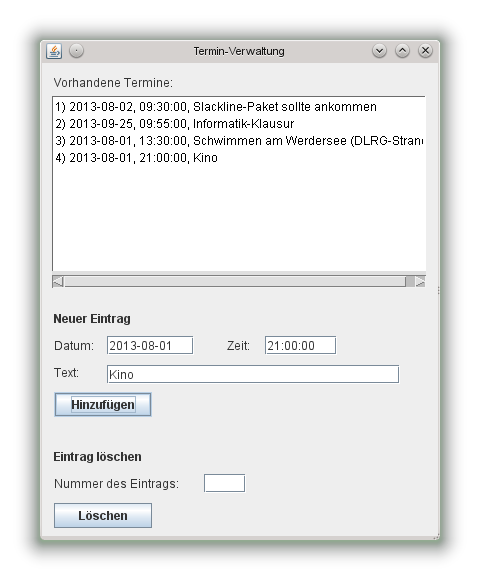
\includegraphics[width=0.5\textwidth]{./inf/SEKII/37_JavaSQL_Datenbankzugriffe/TermineAufgabe2.png}
\caption{Aufgabe 2: So soll der Terminplaner aussehen}
\label{fig:terminplaner}
\end{figure}


\subsection{Aufgabe 3: Ein Programm zum Anzeigen der aktuellen Termine}

Programmiere ein Java-Programm, das die aktuellen Termine des Benutzers anzeigt.
Dieses Programm könnte später zu den Autostart-Programmen gepackt werden und so
bei jedem Start des Computers automatisch aufgerufen werden. Die Oberfläche des
Termin-Anzeigers soll so aussehen:

\begin{center}
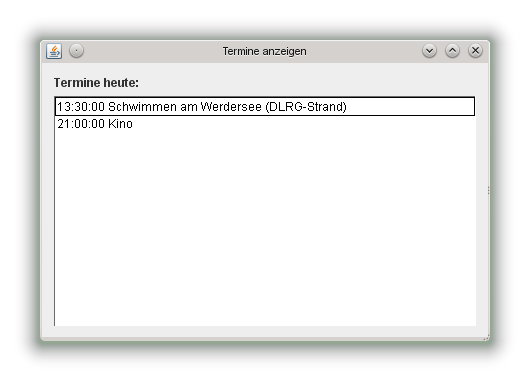
\includegraphics[width=0.5\textwidth]{./inf/SEKII/37_JavaSQL_Datenbankzugriffe/TermineAufgabe3.png}
\end{center}

Der Termin-Anzeiger zeigt die Termine des aktuellen Tages in einer
\myClass{JList}-Komponente an. Die Termine werden aufsteigend nach der Zeit
sortiert. 

Außerdem löscht er unbemerkt vom Benutzer alle Termine aus der Datenbank, die
vor dem aktuellen Datum liegen.

Gib im ersten Schritt das heutige Datum (’\todayI’) fest als String in die
benötigten SQL-Kommandos ein. Hole dir im zweiten Schritt die aktuelle
System-Zeit von der Java-Klasse \myClass{System} mit der statischen Methode
\lstinline|currentTimeMillis()| (also durch Aufruf von
\lstinline|System.currentTimeMillis()|). Übergib diese Zeit an ein Objekt der
Klasse \myClass{Date} aus dem Package \myPackage{java.sql} (Achtung: es gibt
auch eine Klasse \myClass{Date} im Package \myPackage{java.util}!) und lass dir
von der Klasse \myClass{Date} ein \myClass{String}-Objekt mit dem aktuellen Datum
generieren.
